\documentclass{article}
\usepackage[margin=1in]{geometry}
\usepackage{microtype}
\usepackage{setspace}
\usepackage{amsmath}
\usepackage{parskip}
\usepackage{amssymb}
\usepackage{graphicx}

\graphicspath{{../public/}}

\parskip=4ex
\date{}
\author{}

\title{11.7 Maximum and Minimum Values}

\begin{document}
    \maketitle
    A function of two variables has a local maximum at $ (a,b) $ if $ f(x,y) \le f(a,b) $ when $ (x,y) $ is near $ (a,b) $. In the opposite case when $ f(x,y) ge f(a,b) $, then $ f(a,b) $ is a local minimum.

    If the inequalities hold for all points $ (x,y) $ in the domain of $ f $ or $ \{ (x,y)|(x,y) \in D \} $, then $ f $ has an absolute maximum or minimum at $ (a,b) $.

    \textbf{Theorem 12.2}\\
    If $ f $ has a local maximum or minimum at $ (a,b) $ and the first-order partial derivatives of $ f $ exist there, then $ f_{x}(a,b)=0 ~\&~ f_{y}(a,b) =0$.

    A point $ (a,b) $ is called a critical point (or stationary point), $ c $, of $ f $ if $ f_x(a,b)=0 ~\&~ f_y(a,b)=0 $ 

    \textbf{Ex 1}\\
    Let $ f(x,y) =x^{2}+y^{2}-2x-6y+14 $. Then
    \[
        f_{x}=2x-2 \qquad f_{y}(x,y)=2y-6  
    \]

    These partial derivatives are equal to $ 0 $ at the point $ (1,3) $. So the only critical point is $ (1,3) $. By completing the square, we find that
    \[
        f(x,y)=4+(x-1)^{2}+(y-3)^{2}  
    \]

    Since $ (x-1)^{2} \ge 0 ~\&~ (y-3)^{2} \ge 0 $, we have $ f(x,y) \ge 4 $ for all values of $ x ~\&~ y $, therefore $ f(x,y) \ge 4$ for all values of $ x ~\&~ y $. Then not only is $ f(1,3)=4 $ is a local minimum, it is also an absolute minimum. This can be verified by the graph below.
    \begin{center}
        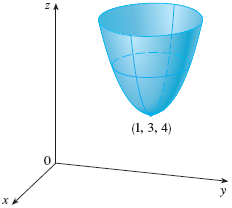
\includegraphics[width=6cm]{11_7_1}
    \end{center}
    
    \textbf{Ex 2}\\
    Find the extreme values of $ f(x,y)=y^{2}-x^{2}. $
    \[
        \begin{gathered}
        f_{x}=-2x \qquad f_{y}=2y\\
        \end{gathered}
    \]
    
    The only critical point is $ (0,0) $. Notice that the points on the $ x $  axis where $ y=0 $. 
    \[
        f(x,y)=-x^{2}<0~(x\neq 0)\\ 
    \]
    The same can be said for points on the $ y $ axis where $ x=0 $
    \[
        f(x,y)=y^{2}>0~(x\neq 0) 
    \]
    Since every disk with the center $ (0,0) $ contains points where $ f $ takes on both positive and negative values. Then $ f(0,0)=0 $ can't be an extreme value so $ f $ does not have any extremas.
   
    \textbf{Second Derivatives Test}\\
    Suppouse the second partial derivatives of $ f $ are continuous on a disk with center $ (a,b) $ and supppouse that $f_x(a,b)=0 ~\&~ f_y(a,b)=0$ (that is, $ (a,b) $ is a critical point of $ f $.) Let
    \[
      D=D(a,b)=f_{xx} (a,b)f_{yy} (a,b)-[f_{xy} (a,b)]^{2} 
    \]

    a) If $ D>0 ~\&~ f_{xx} (a,b)>0$, then $ f(a,b) $ is a local minimum.
    b) If $ D>0 ~\&~ f_{xx} (a,b)<0 $, then $ f(a,b) $ is a local maximum.
    c) If $ D<0 $, then $ f(a,b) $ is not a local maximum or minimum.

    \textbf{Note 1}\\
    In case $ c $, the point $ (a,b) $ is called a saddle point of $ f $ and the graph of $ f $ crosses its tangent plane at $ (a,b) $.

    \textbf{Note 2}\\
    If $ D=0 $, the test gives no information therefore $ f $ could have either a local maximum or minimum at $ (a,b) $. There is also the case that $ (a,b) $ could be a saddle point of $ f $.

    \textbf{Note 3}\\
    $ D $ could also be written as a determinant
    \[
      D = \begin{vmatrix}
       f_{xx} &f_{xy} \\
       f_{yx} &f_{yy}  
      \end{vmatrix} = f_{xx}f_{yy} -(f_{xy})^{2}
    \] 
    
    \textbf{Ex 3}\\
    Find the local maximum and minimum values and saddle points of $ f(x,y) =x^{4}+y^{4}-4xy+1  $
    \[
      \begin{gathered}
      f_x=4x^{3}-4y \qquad f_y = 4y^{3}-4x  
      \end{gathered}
    \]

    We now have the critical points, next we set them to zero to obtain the equations
    \[
      x^{3}-y=0 \qquad y^{3}-x=0  
    \]

    To solve we substitute $ y=x^{3} $ from the first equation into the second one.
    \[
      \begin{gathered}
        (x^{3})^{3} - x = x^{9}-x = x(x^{8}-1)= x(x^{4}-1)(x^{4}+1)\\
        x(x^{2}-1)(x^{2}+1)(x^{4}+1) = x(x-1)(x+1)(x^{2}+1)(x^{4}+1)\\
        x=0,1,-1,~x \in \mathbb{R}\\
      \end{gathered}
    \]
    We now have the real roots $ x=0,1, ~\&~ -1 $. Now we can find the three crtical points
    \[
      \begin{gathered}
      x^{3}=y\\
      ~\\
      -1=-1 \to (-1,-1) \qquad 0=0 \to (0,0) \qquad 1=1 \to (1,1)
      \end{gathered}
    \]

    We now calculate the second partial derivaties and $ D(x,y) $
    \[
      \begin{gathered}
      f_{xx}=24x^{2} \qquad f_{yy}=24y^{2} \qquad f_{xy}=-4\\
      ~\\
      D(x,y)=f_{xx}f_{yy}-(f_{xy})^{2}=144x^{2}y^{2}-16\\
      ~\\
      D(-1,-1)=144(-1)^{2}(-1)^{2}-16=128 \qquad f_{xx}(-1,-1)=12(-1)^{2}=12\\
      D(0,0)=144(0)^{2}(0)^{2}-16 = 16\\
      D(1,1)=144(1)^{2}(1)^{2}-16 = 128 \qquad f_{xx}(1,1)=12(1)^{2}=12
      \end{gathered}
    \]
    $ D(-1,1) >0 ~\&~ f_{xx}(-1,-1)=12>0 $, then $ f(-1,-1) $  Since $ D(0,0)=-16<0$, then the origin $ (0,0) $ is a saddle point and $ f $ has no extrema values at the origin.

    \textbf{Ex 4}\\
    Find the shortest distance from the point $ (1,0,-2) $ to the plane $ x+2y+z=4 $
    \[
      \begin{gathered}
      x+2y+z=4 \to z=4-x-2y\\
      ~\\
      d=\sqrt{(x-1)^{2}+y^{2}+(z+2)^{2}} \to d=\sqrt{(x-1)^{2}+y^{2}+(6-x-2y)^{2}}\\
      ~\\
      d^{2}=f(x,y)=(x-1)^{2}+y^{2}+(6-x-2y)^{2}\\
      ~\\
      f_x=2(x-1)-2(6-x-2y)=4x+4y-14=0 \qquad f_y=2y-4(6-x-2y)=4x+10y-24=0\\
      ~\\
      4x+4y-14 = 0 \to y=-x+\frac{14}{4}\\
      4x+10y-24=0 \to 4x+10(-x+\frac{14}{4})-24=0\\
      4x-10x+\frac{140}{4}-\frac{96}{4}\to -6x+\frac{44}{4}=0\\
      -6x=-11\\
      x=\frac{11}{6}\\
      ~\\
      y=-x+\frac{14}{4}\to y=-\frac{11}{6}+\frac{14}{4}\\
      y=\frac{40}{24}\to \frac{5}{3}\\
      ~\\
      c=(x,y)=(\frac{11}{6},\frac{5}{3})\\
      ~\\
      f_{xx}=4 \qquad f_{yy}=10 \qquad f_{xy}=4\\
      ~\\
      D(x,y)=f_{xx}f_{yy}-(f_{xy})^{2}\\
      D(\frac{11}{6},\frac{5}{3} ) = 4\cdot 10 - 16=24>0 \qquad f_{xx}=4>0   
      \end{gathered}
    \]

    Now because $ D =24>0 ~\&~ f_{xx}=4>0$, then the critical point $ c= (\frac{11}{6},\frac{5}{3}) $, then the critical point $ c $ is a local minimum. Intuitively, because there is only one critical point, then the local minimum must be an absolute minimum.
  \[
    \begin{gathered}
        d=\sqrt{(x-1)^{2}+y^{2}+(6-x-2y)^{2}} = \sqrt{(\frac{11}{6}-\frac{6}{6})^{2}+(\frac{5}{3})^{2}+(\frac{36}{6}-\frac{11}{6}-\frac{10}{3})^{2}}\\
        ~\\
      d=\sqrt{(\frac{5}{6})^{2}+(\frac{5}{3})^{2}+(\frac{5}{6})^{2}}=\boxed{\frac{5\sqrt{6}}{6}} 
    \end{gathered}
  \]

  \textbf{Ex 5}\\
  A rectangular box without a lid is to be made from $ 12m^{2} $ of cardboard. Find the maximum volume of such a box.
  \begin{center}
    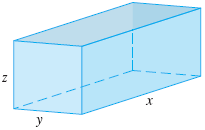
\includegraphics[width=4cm]{11_7_2}
  \end{center}
  \[
    \begin{gathered}
    V=xyz \qquad x=\text{length},y=\text{width},z=\text{height}\\
    \end{gathered}
  \]
  
  The 3 areas composing of an open lid box can be represented as so
  \[
    A_1=xz \qquad A_2 = yz \qquad A_3 = yx
  \]

  Since the cardboard was made from $ 12m^{2} $ of cardboard, the surface area is $ 12m^{2} $, we get the equation
  \[
    2A_1 + 2A_2+yx=12 \to 2xz +2yz+yx=12
  \]
  By solving for $ z $ we get the equation
  \[
    \begin{gathered}
      2xz+2yz+xy=12 \to 2xz+2yz=12xy-xy\\
      2z(x+y)=12-xy \to z=\frac{12xy-xy}{2(x+y)}\\
      ~\\
      V=xyz \to V=xy\frac{12-xy}{2(x+y)} \to \frac{12xy-x^{2}y^{2}}{2(x+y)}
    \end{gathered}
  \]

  The reason being that $ z $ becomes a function of $ x ~\&~ y $ so $ z=f(x,y)$. We now compute the partial derivatives
  \[
    \begin{gathered}
    \frac{\partial V}{\partial x}=f_x=\frac{y^{2}(12-2xy-x^{2})}{2(x+y)^{2}} \qquad
    \frac{\partial V}{\partial y}=f_y=\frac{x^{2}(12-2xy-y^{2})}{2(x+y)^{2}}
    \end{gathered}
  \]

  If $ V $ is a maximum, then the critical points $ \frac{\partial V}{\partial x}=0 ~\&~ \frac{\partial V}{\partial y}=0$, but $ x=0 ~\&~ y=0 $ makes the equation $ V=xyz\to0 $. So we must solve the equations
  \[
    \begin{gathered}
    12-2xy-x^{2}=0 \qquad 12-2xy-y^{2}=0\\
    x^{2} = 12-2xy \qquad y^{2}=12-2xy 
    \end{gathered}
  \]

  These equations imply that $ x^{2}=y^{2} \to |x|=|y|$, indicating that not only $ x=y $ but $ \{ x,y \in \mathbb{R} \} $.
  \[
    \begin{gathered}
    y=x\\  
    x^{2}=12-2xy \to x^{2}= 12-2x^{2} \to 3x^{2}=12\\
    x^{2}=4 \to x^{2}=2\\
    ~\\
    x=y\\
    y^{2}=12-2xy \to y^{2}=12-2yy \to 3y^{2}=12\\
    y^{2}=4 \to y=2\\
    ~\\
    x=2,y=2,z=\frac{12xy-x^{2}y^{2}}{2(x+y)}
    ~\\
    z=\frac{12xy-x^{2}y^{2}}{2(x+y)}\to \frac{12(4)-16}{2(4)}=1\\
    ~\\
    c=(x,y,z)=(2,2,4) 
    \end{gathered}
  \]

  From the physical nature of the problem, $ (x,y,z) $ can be argued to be an absolute maximum volume occuring at the critical point, $ c=(2,2,1) $ of $ V $. Then
  \[
  V=xyz\to2 \cdot 2 \cdot 1 = 4m^{3}  
  \]
  
\end{document}
